\documentclass[12pt,reqno,a4paper,oneside,draft]{article}

\usepackage{amsmath,amssymb,amsthm}
\usepackage[english]{babel}
\usepackage[utf8]{inputenc}
\usepackage[T1]{fontenc}

\usepackage{graphicx}

\theoremstyle{plain}
\newtheorem{thm}{Theorem}[section]
\newtheorem{lem}[thm]{Lemma}
\newtheorem{prop}[thm]{Proposition}
\newtheorem{cor}[thm]{Corollary}

\theoremstyle{definition}
\newtheorem*{defn}{Definition}
\newtheorem{exmp}{Example}[section]

\theoremstyle{remark}
\newtheorem*{rem}{Remark}

\begin{document}

\tableofcontents


\section{Introduction}
\label{sec:Introduction}
A problem of lifetime distribution estimation from randomly right-censored observations naturally appears in actuarial and medical statistics as well as in device reliability analysis $\#$. In case of independent identically distributed observations \emph{Kaplan-Meier estimator} is usually used $\#$. Consider a model in which each observation is drawn from a finite mixture of distributions. If mixture probabilities (concentrations) varies through the observations, this model is called \emph{mixture model with varying concentrations}. A modification of Kaplan-Meier estimator for this model has already been discussed by V. Khizanov, R. Maiboroda and A. Ryzhov in papers $\#$. In this paper two different estimators (modifications) are compared via numerical simulations.

The problem statement is formulated in Section \ref{sec:Problem_statement}. Sections \ref{sec:Simulation_description} and \ref{sec:Simulation_results} are devoted to description and results of simulations respectively. Conclusions are presented in Section \ref{sec:Conclusions}.

\section{Problem statement}
\label{sec:Problem_statement}
Let $\mathcal O = \{O_j\}_{j=1}^n$ be a sample from mixture model with varying concentrations. Each $O_j$ belongs to one of $M$ components which is denoted by $\mathrm{ind}(O_j)$. Suppose that the true value of $\mathrm{ind}(O_j)$ is not observed. Instead, one is provided with \emph{mixture probabilities}
\begin{equation}
\label{eq:mixture_probabilities}
w_j^m = \mathbb P(\mathrm{ind}(O_j) = m), \, m=1,\ldots, M
\end{equation}
For each object $O_j$ there exists a positive characteristic $\xi _j = \xi (O_j)$ which is treated as a lifetime. Distribution of each $\xi _j$ depends on the component it belongs to, i.e.:
\begin{equation}
\label{eq:conditional_distribution}
F_m (A) = \mathbb P(\xi _j \in A \mid \mathrm{ind}(O_j) = m), \, m=1,\ldots , M
\end{equation}
\begin{rem}
Mixture probabilities \eqref{eq:mixture_probabilities} satisfy normalization property
\begin{equation}
\label{eq:mix_prob_constraint}
\sum _{m=1}^M w_j^m = 1, \, j = 1,\ldots, n
\end{equation}
\end{rem}

Consider the case in which \emph{true data} $\mathcal D = \{\xi _j\}_{j=1}^n$ are randomly right-censored. That is there exists a sequence of positive random variables $\{c_j\}_{j=1}^n$ such that only \emph{censored data} $\mathcal D^c = \{(\xi _j^*, \delta _j)\}_{j=1}^n$, where $\xi _j^* = \min (\xi _j, c_j)$ and $\delta _j = \mathbf 1\{\xi _j \leq c_j\}$ for each $j=1,\ldots ,n$, are observed. Here, $c_j$'s are called \emph{censors} and their conditional distributions are given by:
\begin{equation}
G_m (A) = \mathbb P(c _j \in A \mid \mathrm{ind}(O_j) = m),\, m=1,\ldots , M
\end{equation} 

One problem is to estimate conditional distributions $\{F_m\}_{m=1}^M$ from censored data $\mathcal D^c$ and mixture probabilities $\mathbf W = (w_j^m)_{j,m=1}^{n,M}$. Vectors $(\xi _j, c _j)$ are assumed to be independent as well as variables $\xi _j$ and $c_j$ are conditionally independent given $\mathrm{ind}(O_j)$ for each $j=1,\ldots ,n$. Two solutions for this problem are proposed in subsequent sections. For the sake of simplicity only cumulative distribution functions are considered.

\subsection{Ryzhov estimator}
\label{subsec:ryzhov_estimator}
Suppose a data set $\tilde {\mathcal D}$ is divided by $N$ subsamples $\{\tilde{\mathcal D} _i\}_{i=1}^N$ where each subsample $\tilde{\mathcal D}_i$ comprises i.i.d. random variables $\{\xi _{j_i} \}_{j_i=1}^{n_i}$ with the following CDF:
\begin{equation}
\label{eq:Ryzhov_mixture_distribution}
H_i(t) = \mathbb P(\xi _{j_i} \leq t) = \sum _{m=1}^M w_i^mF_m(t), \, i = 1,\ldots, N,
\end{equation}
where $w_i^m$ and $F_m$ are defined by \eqref{eq:mixture_probabilities} and \eqref{eq:conditional_distribution} respectively. Censors $\{c_{j_i} \}$ are introduced in the same spirit and together with $\{\xi _{j_i}\}$ form censored data $\tilde{\mathcal D}^c$.

In order to estimate conditional distributions $\{F_m\}_{m=1}^M$ in this settings Ryzhov's estimator can be applied $\#$. It is defined in two steps: first one should estimate each $H_i$ by applying Kaplan-Meier estimator to each subsample $\tilde{\mathcal D}^c_i$, and then use these estimations for deriving $\hat F_m$. That is
\begin{equation}
\hat H^{\mathrm{KM}}_i (t) = 1 - \prod _{j_i:\xi ^*_{j_i} \leq t} \Bigg(1 - \frac {\delta _{j_i}}{n_i - j_i + 1}\Bigg)
\end{equation}
and
\begin{equation}
\label{eq:ryzhov_estimator}
\hat F^{\mathrm{R}}_m(t) = \sum _{i=1}^N a_i^m \hat H^{\mathrm{KM}}_i(t),
\end{equation}
where coefficients $a_i^m$ are determined by the $mi$-th element of a matrix
\begin{equation}
(\mathbf W^\top \boldsymbol{\Sigma}^{-1}\mathbf W)^{-1} \mathbf W^\top \boldsymbol{\Sigma}^{-1}
\end{equation}
Here, $\boldsymbol{\Sigma} = \mathbf{diag}(\mathbb V [\hat H^{\mathrm{KM}}_1], \ldots, \mathbb V[\hat H^{\mathrm{KM}}_N])$ denotes the variance of Kaplan-Meier estimator. As long as it depends on unknown distributions $H_1, \ldots, H_N$ one can use Greenwood's formula in order to estimate it:
\begin{equation}
\hat{\mathbb V}[\hat H^{\mathrm{KM}}_i] = (1 - \hat H^{\mathrm{KM}}_i)^2 \sum _{j_i:\xi _{j_i} \leq t}\frac {\delta _{j_i}}{(n_i - j_i)(n_i - j_i + 1)}
\end{equation}
\begin{thm}[Ryzhov]
Suppose all $n_i = O(n)$, where $n = n_1 + \ldots + n_N$ and mixture probability matrix $\mathbf W$ has full rank. Then $\hat F^R_m$ defined by \eqref{eq:ryzhov_estimator} is uniformly consistent and asymptotically normal estimator of $F_m$ for each $m=1,\ldots , M$.
\end{thm}


\subsection{Khizanov-Maiboroda estimator}
Since Ryzhov's estimator suffers from some drawbacks described in previous section one can use an estimator proposed by V. Khizanov and R. Maiboroda $\#$. This estimator takes the form:
\begin{equation}
\label{eq:khizanov_maiboroda_estimator}
\hat F^{\mathrm{KhM}}_m = 1 - \prod _{j : \xi ^*_j \leq t}\bigg( 1 - \frac {a_j^m \delta _j}{1 - \sum _{i:\xi ^*_i < t} a_i^m} \bigg)
\end{equation}
where coefficients $a_j^m$ are equal to $mj$-th element of a matrix
\begin{equation}
(\mathbf W^\top \mathbf W)^{-1}\mathbf W^\top
\end{equation}
\begin{thm}
Let mixture probability matrix $\mathbf W$ has full rank. Then $\hat F^{\mathrm{KhM}}_m$ defined by \eqref{eq:khizanov_maiboroda_estimator} is uniformly consistent estimator of $F_m$ for each $m=1,\ldots, M$.
\end{thm}
\begin{rem}
Asymptotic normality of Khizanov-Maiboroda's estomator has not been proven yet.
\end{rem}



\section{Simulation description}
\label{sec:Simulation_description}
This section introduces settings for comparison of two estimators described in previously. Since Ryzhov's estimator requires a special form of input  only $\tilde{\mathcal D}$ data described in \ref{subsec:ryzhov_estimator} are considered. That is, mixture probability matrix $\mathbf W$ for Khizanov-Maiboroda's estimator is obtained by replicating each $i$-th row of respective matrix $n_i$ times for $i=1,\ldots, N$.

For each experiment mixture probability matrix is drawn uniformly from the set of all matrices which satisfy normalization property \eqref{eq:mix_prob_constraint}. In order to prevent ill-conditioned cases only matrices with $\det (\mathbf W^\top \mathbf W) > 0.2$ are considered. For the sake of simplicity all $n_i,i = 1,\ldots, N$ are assumed to be equal and further denoted simply by $n$. Next section provides simulation results for two-component mixture, i.e. $M=2$, where the quantity
\begin{equation}
\mathbb E \sup _{t} |\hat F_m(t) - F_m(t)|, \, m=1,2
\end{equation}
is compared for different values of $n$ and $N$.

\section{Simulation results}
\label{sec:Simulation_results}
Let $F_1\sim \chi ^2_1$ and $F_2\sim \chi ^2_2$ have chi-squared distribution with parameters $1$ and $2$ respectively. All censors $c_j$ have the same uniform distribution $G\sim \mathcal U(0, 8)$ which corresponds to approximately $20\%$ of censored observations. Consider the case in which $N=2$ is fixed while $n$ varies from $100$ to $1000$. Figure \ref{fig:1} illustrates that an error of each estimator becomes almost equal as $n$ increases.
\begin{figure}
\centering
\caption{\label{fig:1}Error comparison for fixed number of subsamples $N=2$. 1000 iterations are used for estimating expectation of supremum error.}
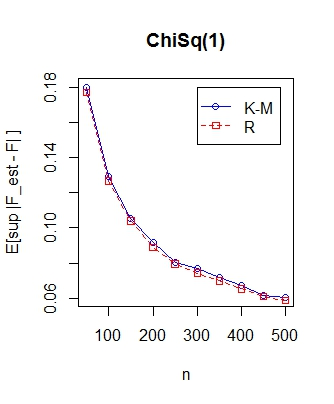
\includegraphics[scale=0.55]{ChiSq1_n.jpeg}
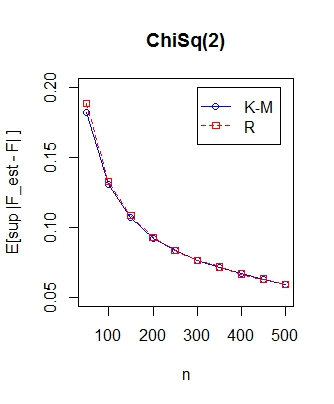
\includegraphics[scale=0.55]{ChiSq2_n.jpeg}
\end{figure}


However, if one fixes $n=50$ and varies $N$ from $2$ to $20$ then Khizanov-Maiboroda's estimator starts to outperform Ryzhov's estimator as $N$ increases. This can be noticed in Figure \ref{fig:2}.
\begin{figure}
\centering
\caption{\label{fig:2}Error comparison for fixed number of observations in each subsample $n=50$. 1000 iterations are used for estimating expectation of supremum error.}
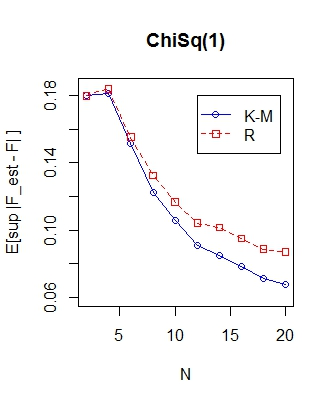
\includegraphics[scale=0.55]{ChiSq1_G.jpeg}
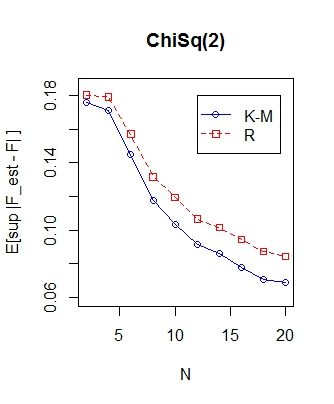
\includegraphics[scale=0.55]{ChiSq2_G.jpeg}
\end{figure}



\section{Conclusions}
\label{sec:Conclusions}
...


\end{document}
